\documentclass[pdflatex,compress]{beamer}

%\usetheme[dark,framenumber,totalframenumber]{ElektroITK}
\usetheme[darktitle,framenumber,totalframenumber]{ElektroITK}
\usepackage{graphicx}
\usepackage{multicol}

\title{Data Communications}
\subtitle{Chapter 5 - Signal Encoding Techniques}

\author{Mifta Nur Farid}

\begin{document}

\maketitle

\begin{frame}
	\frametitle{Encoding and Modulation}
	\begin{center}
		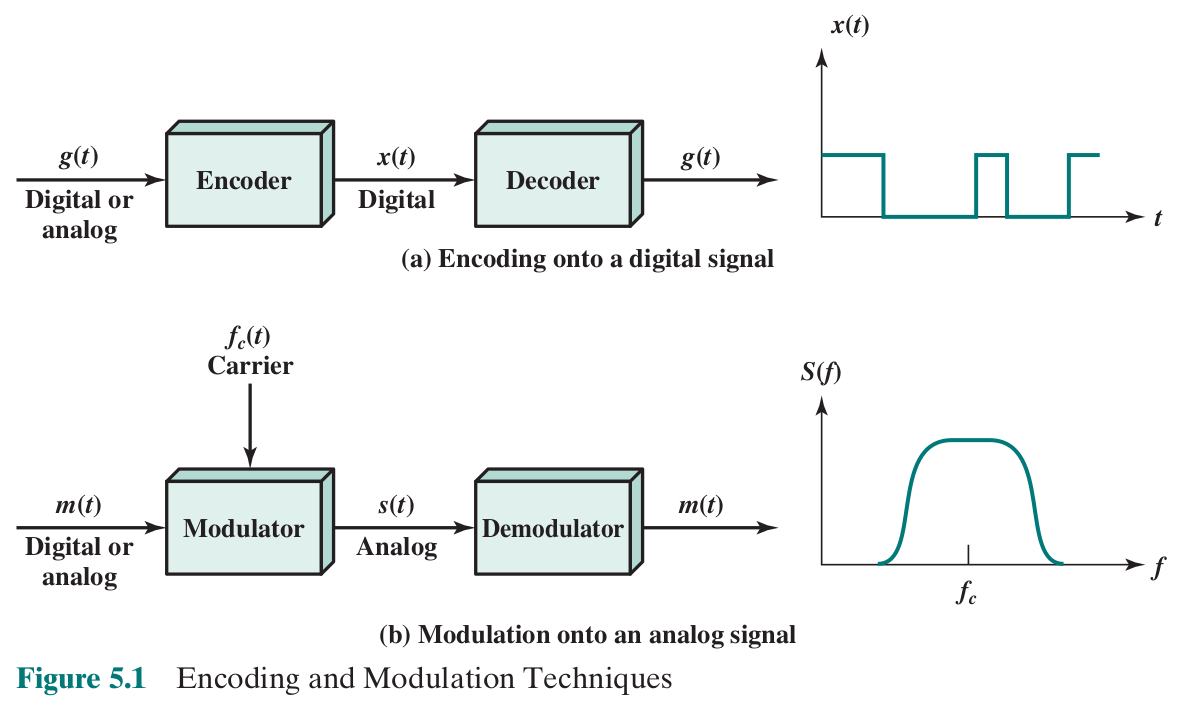
\includegraphics[width=\linewidth]{img/img01}
	\end{center}
\end{frame}

\begin{frame}
	\frametitle{Digital Data, Digital Signal}
	\textbf{Digital signal}
	\begin{itemize}
		\item Sequence of discrete, discontinuous voltage pulses
		\item Each pulse is a signal element
		\item Binary data are transmitted by encoding each data bit into signal elements
	\end{itemize}
\end{frame}

\begin{frame}
	\frametitle{Terminology}
	\begin{itemize}
		\item \textbf{Unipolar}: all signal elements have the same sign
		\item \textbf{Polar}: one logic state represented by positive voltage and the other by negative voltage
		\item \textbf{Data rate}: rate, in bits per second that data are transmitted
		\item \textbf{Duration or length of a bit}: time taken for transmitter to emit the bit
		\item \textbf{Modulation rate}: rate at which the signal level is changed; the rate is expressed in baud, which means signal elements per second
		\item \textbf{Mark and space}: refer to the binary digits 1 and 0
	\end{itemize}
\end{frame}

\begin{frame}
	\frametitle{Key Data Transmission Terms}
	\begin{center}
		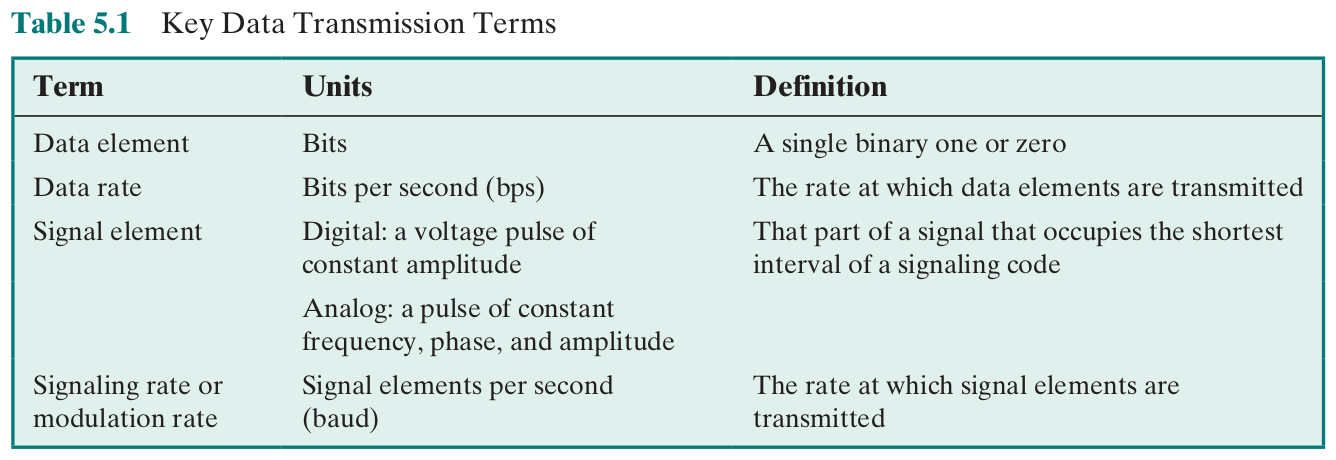
\includegraphics[width=\linewidth]{img/img02}
	\end{center}
\end{frame}

\begin{frame}
	\frametitle{Interpreting Signals}
	\begin{multicols}{2}
		\begin{itemize}
			\centering
			\item[] \textbf{Tasks involved in interpreting digital signal at the receiver:}\\
			\centering $ \downarrow $
			\item[] Timing of bits - when they start and end\\
			\centering $ \downarrow $
			\item[] Signal levels
		\end{itemize}
	\columnbreak
		\begin{itemize}
			\centering
			\item[] \textbf{Factors affecting signal interpretation:}\\
			\centering $ \downarrow $
			\item[] Signal to noise ratio\\
			\centering $ \downarrow $
			\item[] Data rate\\
			\centering $ \downarrow $
			\item[] Bandwidth
		\end{itemize}
	\end{multicols}
\end{frame}

\begin{frame}
	\frametitle{Definition of Digital Signal Encoding Formats}
	\begin{center}
		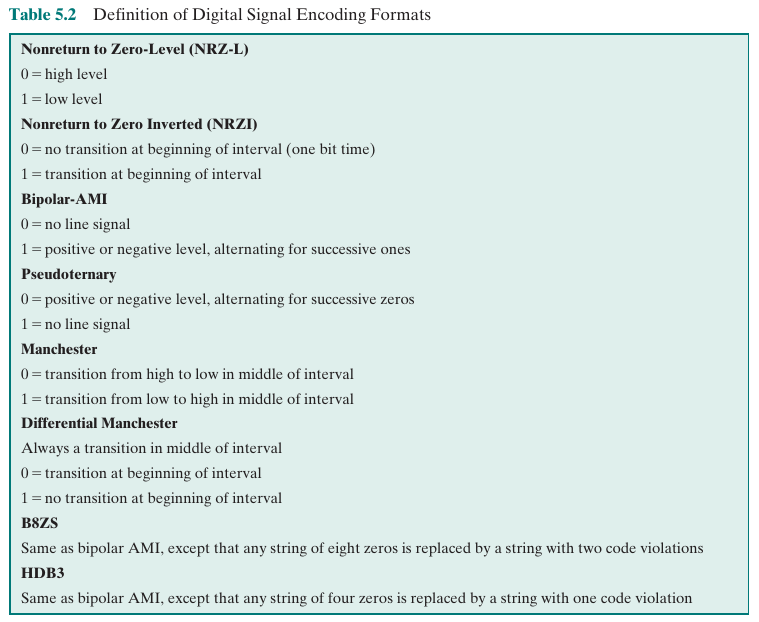
\includegraphics[width=0.7\linewidth]{img/img03}
	\end{center}
\end{frame}

\begin{frame}
	\frametitle{Digital Signal Encoding Formats}
	\begin{center}
		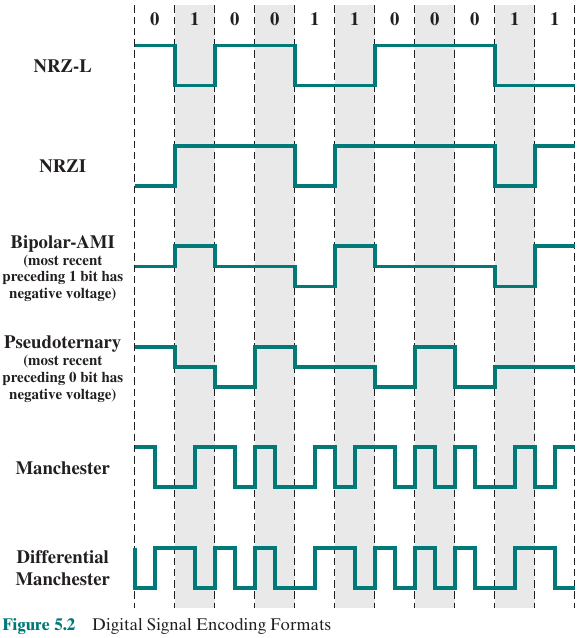
\includegraphics[width=0.6\linewidth]{img/img04}
	\end{center}
\end{frame}

\begin{frame}
	\frametitle{Encoding Schemes}
	\begin{itemize}
		\item \textbf{Signal spectrum}\\
		A good signal design should concentrate the transmitted power in the middle of the transmission bandwidth
		\item \textbf{Clocking}\\
		Need to synchronize transmitter and receiver either with an external clock or sync mechanism
		\item \textbf{Error detection}\\
		Responsibility of a layer of logic above the signaling level that is known as data link control
		\item \textbf{Signal interference and noise immunity}\\
		Certain codes perform better in the presence of noise
		\item \textbf{Cost and complexity}\\
		The higher the signaling rate the greater the cost
	\end{itemize}
\end{frame}

\begin{frame}
	\frametitle{Nonreturn to Zero}
	\begin{itemize}
		\item Easiest way to transmit digital signals is to use two different voltages for 0 and 1 bits
		\item Voltage level is constant during a bit interval
		\begin{itemize}
			\item No transition (no return to a zero voltage level)
			\item Absence of voltage for 0, constant positive voltage for 1
			\item More often, a negative voltage represents one value and a positive voltage represents the other (NRZ-L)
		\end{itemize}
	\end{itemize}
\end{frame}

\begin{frame}
	\frametitle{Non-return to Zero Inverted (NRZI)}
	\begin{itemize}
		\item Non-return to zero, invert on ones
		\item Maintains a constant voltage pulse for duration of a bit time
		\item Data are encoded as presence or absence of signal transition at the beginning of the bit time
		\begin{itemize}
			\item Transition (low to high, high to low) denotes binary 1
			\item No transition denotes binary 0
		\end{itemize}
		\item Is an example of differential encoding
		\begin{itemize}
			\item Data are represented by changes rather than levels
			\item More reliable to detect a transition in the presence of noise than to compare a value to a threshold
			\item Easy to lose sense of polarity
		\end{itemize}
	\end{itemize}
\end{frame}

\begin{frame}
	\frametitle{Spectral Density of Various Signal Encoding Schemes}
	\begin{center}
		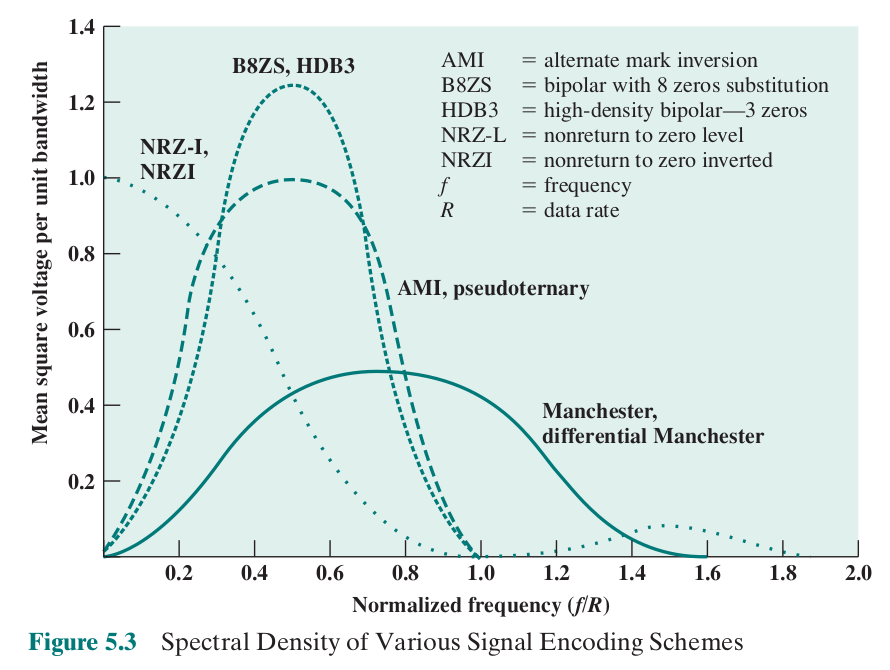
\includegraphics[width=0.8\linewidth]{img/img05}
	\end{center}
\end{frame}

\begin{frame}
	\frametitle{Multilevel Binary Bipolar-AMI}
	\begin{itemize}
		\item Use more than two signal levels
		\item Bipolar-AMI
		\begin{itemize}
			\item Binary 0 represented by no line signal\\
			Binary 1 represented by positive or negative pulse
			\item Binary 1 pulses alternate in polarity
			\item No loss of sync if a long string of 1s occurs
			\item No net dc component
			\item Lower bandwidth
			\item Easy error detection
		\end{itemize}
	\end{itemize}
\end{frame}

\begin{frame}
	\frametitle{Multilevel Binary Pseudoternary}
	\begin{itemize}
		\item Binary 1 represented by absence of line
		signal (zero voltage)
		\item Binary 0 represented by alternating positive and negative pulses
		\item No advantage or disadvantage over bipolar-AMI and each is the basis of some applications
	\end{itemize}
\end{frame}

\begin{frame}
	\frametitle{Multilevel Binary Issues}
	\begin{itemize}
		\item Synchronization with long runs of 0’s or 1’s
		\begin{itemize}
			\item Can insert additional bits that force transitions
			\item Scramble data
		\end{itemize}
		\item Not as efficient as NRZ
		\begin{itemize}
			\item Each signal element only represents one bit
			\begin{itemize}
				\item Receiver distinguishes between three levels: +A, -A, 0
			\end{itemize}
			\item A 3 level system could represent $ \log_2 (3) = 1.58 $ bits
			\item Requires approximately 3 dB more signal power for same probability of bit error
		\end{itemize}
	\end{itemize}
\end{frame}

\begin{frame}
	\frametitle{Theoretical Bit Error Rate for Various Encoding Schemes}
	\begin{center}
		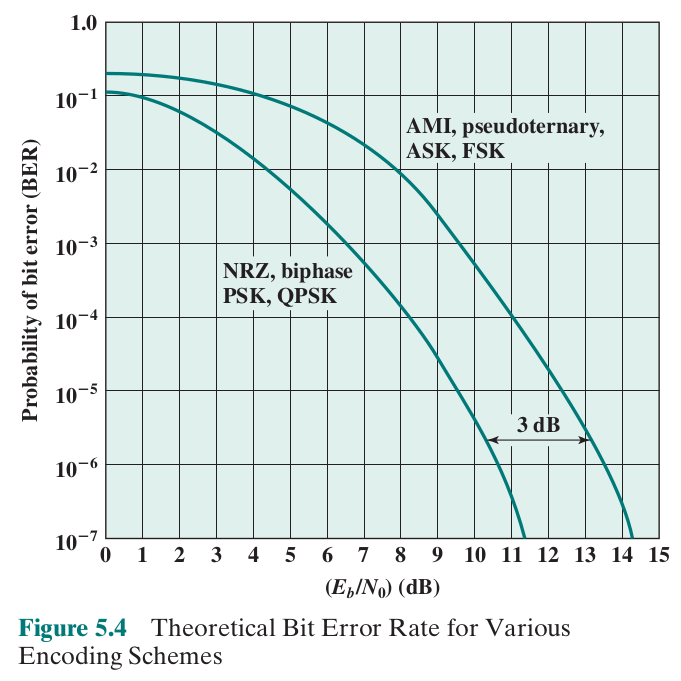
\includegraphics[width=0.6\linewidth]{img/img06}
	\end{center}
\end{frame}

\begin{frame}
	\frametitle{Manchester Encoding}
	\begin{itemize}
		\item There is a transition at the middle of each bit period
		\item Midbit transition serves as a clocking mechanism and also as data
		\item Low to high transition represents a 1
		\item High to low transition represents a 0
	\end{itemize}
\end{frame}

\begin{frame}
	\frametitle{Differential Manchester Encoding}
	\begin{itemize}
		\item Midbit transition is only used for clocking
		\item The encoding of a 0 is represented by the presence of a transition at the beginning of a bit period
		\item A 1 is represented by the absence of a transition at the beginning of a bit period
		\item Has the added advantage of employing differential encoding
	\end{itemize}
\end{frame}

\begin{frame}
	\frametitle{Biphase Pros and Cons}
	\begin{itemize}
		\item Pros
		\begin{enumerate}
			\item Synchronization
			\item No DC component
			\item Has error detection
		\end{enumerate}
		\item Cons
		\begin{enumerate}
			\item At least one transition per bit time and may have two
			\item Maximum modulation rate is twice NRZ
			\item Requires more bandwidth
		\end{enumerate}
	\end{itemize}
\end{frame}

\begin{frame}
	\frametitle{A Stream of Binary Ones at 1 Mbps}
	\begin{center}
		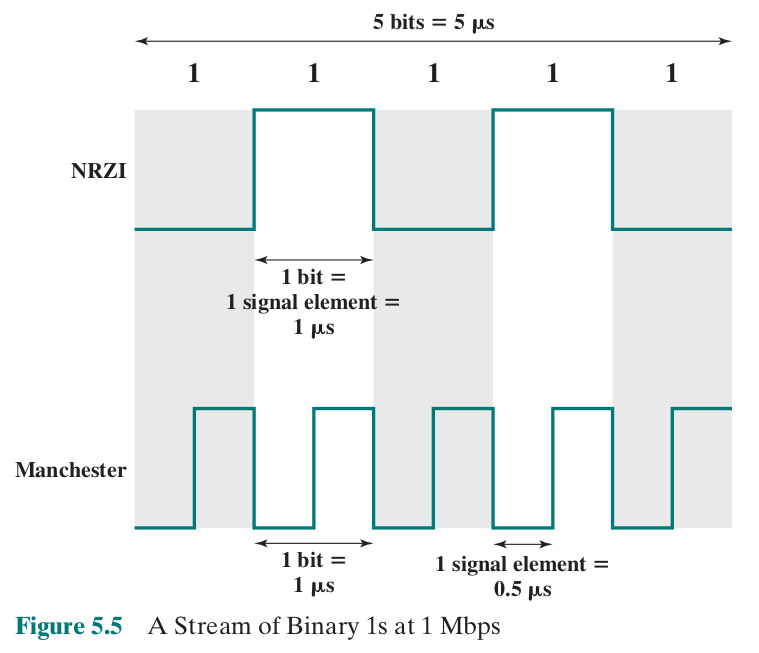
\includegraphics[width=0.7\linewidth]{img/img07}
	\end{center}
\end{frame}

\begin{frame}
	\begin{center}
		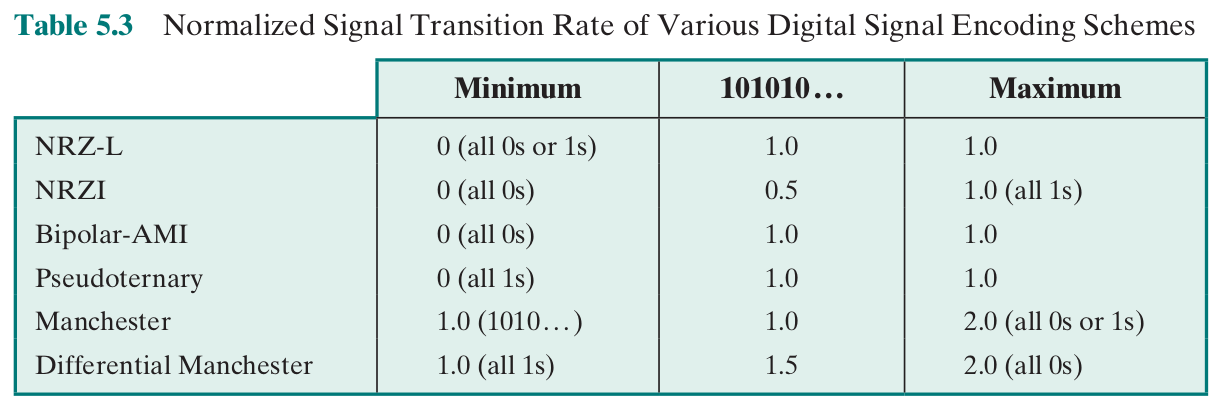
\includegraphics[width=\linewidth]{img/img08}
	\end{center}
\end{frame}

\begin{frame}
	\frametitle{Scrambling}
	\begin{itemize}
		\item Use scrambling to replace sequences that would produce constant voltage
		\item These filling sequences must:
		\begin{itemize}
			\item Provide sufficient transitions for the receiver’s clock to maintain synchronization
			\item Be recognized by the receiver and replaced with the original data sequence
			\item Be the same length as the original sequence so there is no data rate penalty
		\end{itemize}
		\item Design Goals:
		\begin{enumerate}
			\item Have no dc component
			\item Have no long sequences of zero level line signals
			\item Have no reduction in data rate
			\item Error detection capability
		\end{enumerate}
	\end{itemize}
\end{frame}

\begin{frame}
	\frametitle{B8ZS}
	\begin{itemize}
		\item Bipolar with 8-zeros substitution
		\item Coding scheme commonly used in North America
		\item Based on a bipolar-AMI
		\begin{itemize}
			\item Amended with the following rules:
			\begin{itemize}
				\item If an octet of all zeros occurs and the last voltage pulse preceding this octet was positive, then the eight zeros of the octet are encoded as 000+-0-+
				\item If an octet of all zeros occurs and the last voltage pulse preceding this octet was negative, then the eight zeros of the octet are encoded as 000-+0+-
			\end{itemize}
		\end{itemize}
	\end{itemize}
\end{frame}

\begin{frame}
	\begin{center}
		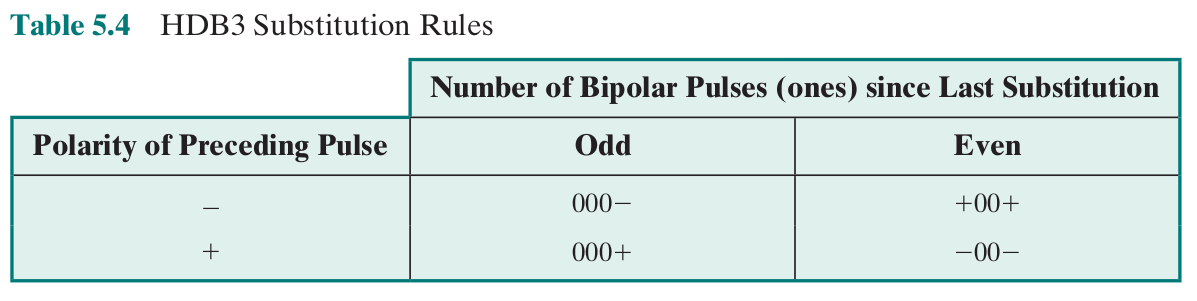
\includegraphics[width=\linewidth]{img/img09}
	\end{center}
	Check if you know why DC is still zero!
\end{frame}

\begin{frame}
	\begin{center}
		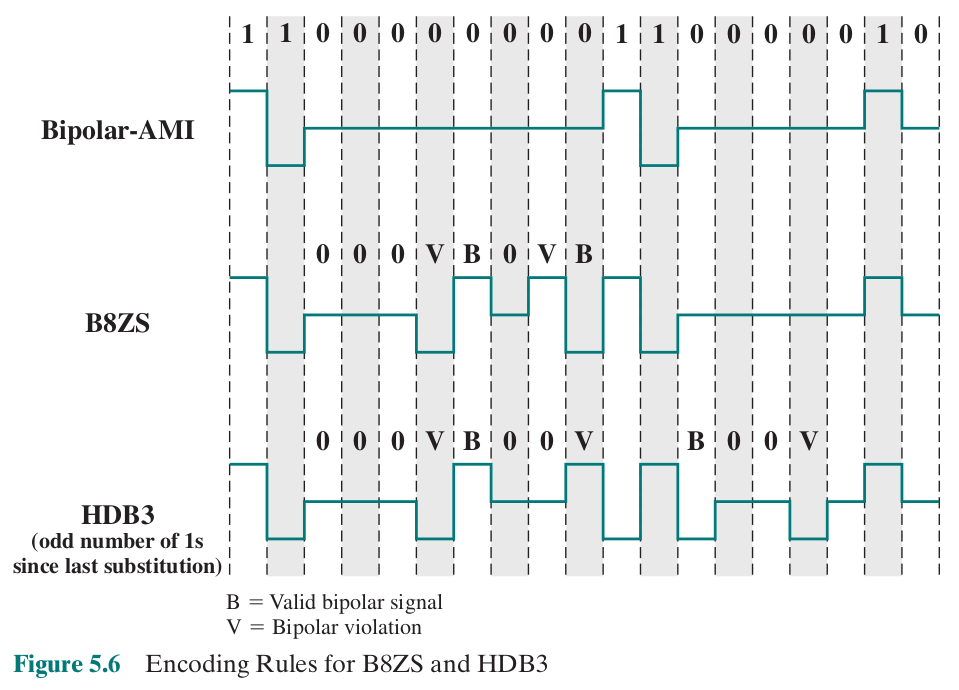
\includegraphics[width=0.9\linewidth]{img/img10}
	\end{center}
\end{frame}

\begin{frame}
	\frametitle{Digital Data, Analog Signal}
	\begin{itemize}
		\item Main use is public telephone system
		\begin{itemize}
			\item Was designed to receive, switch, and transmit analog signals
			\item Has a frequency range of 300Hz to 3400Hz
			\item Is not at present suitable for handling digital signals from the subscriber locations
			\item Uses modem (modulator-demodulator) to convert digital data to analog signals and vice versa
		\end{itemize}
	\end{itemize}
\end{frame}

\begin{frame}
	\begin{center}
		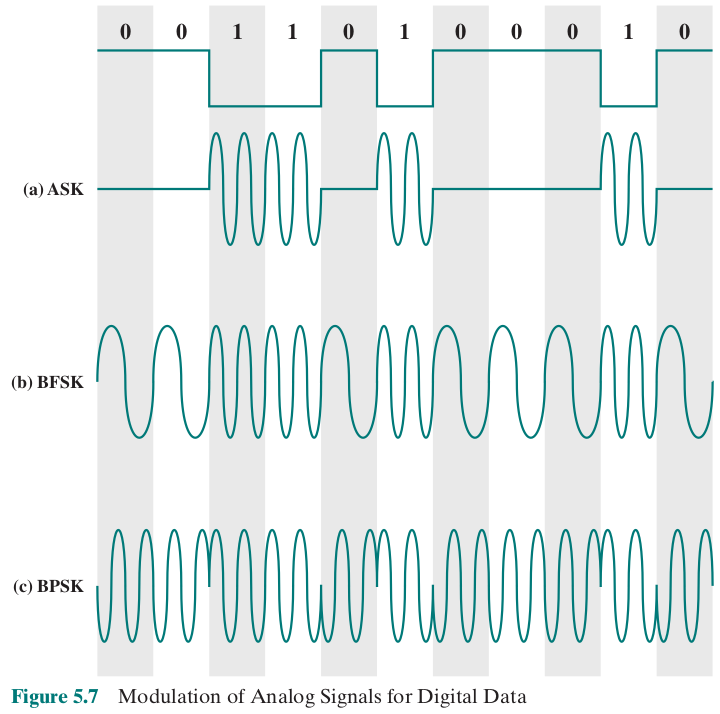
\includegraphics[width=0.6\linewidth]{img/img11}
	\end{center}
\end{frame}

\begin{frame}
	\frametitle{Amplitude Shift Keying (ASK)}
	\begin{itemize}
		\item Encode 0/1 by different carrier amplitudes
		\begin{itemize}
			\item Usually have one amplitude zero
		\end{itemize}
		\item Susceptible to sudden gain changes
		\item Inefficient
		\item Used for:
		\begin{itemize}
			\item Up to 1200bps on voice grade lines
			\item Very high speeds over optical fiber
		\end{itemize}
	\end{itemize}
\end{frame}

\begin{frame}
	\frametitle{Binary Frequency Shift Keying\\(BFSK)}
	\begin{itemize}
		\item Most common form of FSK
		\item Two binary values are represented by two different frequencies (near carrier)
		\item Less susceptible to error than ASK\\
		\item Used for:
		\begin{itemize}
			\item Up to 1200bps on voice grade lines
			\item High frequency radio
			\item Even higher frequency on LANs using coaxial cable
		\end{itemize}
	\end{itemize}
\end{frame}

\begin{frame}
	\begin{center}
		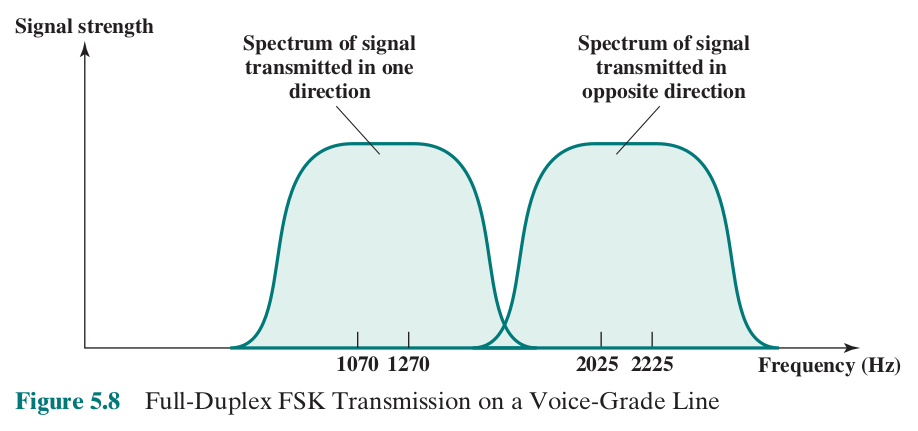
\includegraphics[width=\linewidth]{img/img12}
	\end{center}
\end{frame}

\begin{frame}
	\frametitle{Multiple FSK (MFSK)}
	\begin{itemize}
		\item Each signaling element represents more than one bit
		\item More than two frequencies are used
		\item More bandwidth efficient
		\item More susceptible to error
	\end{itemize}
\end{frame}

\begin{frame}
	\begin{center}
		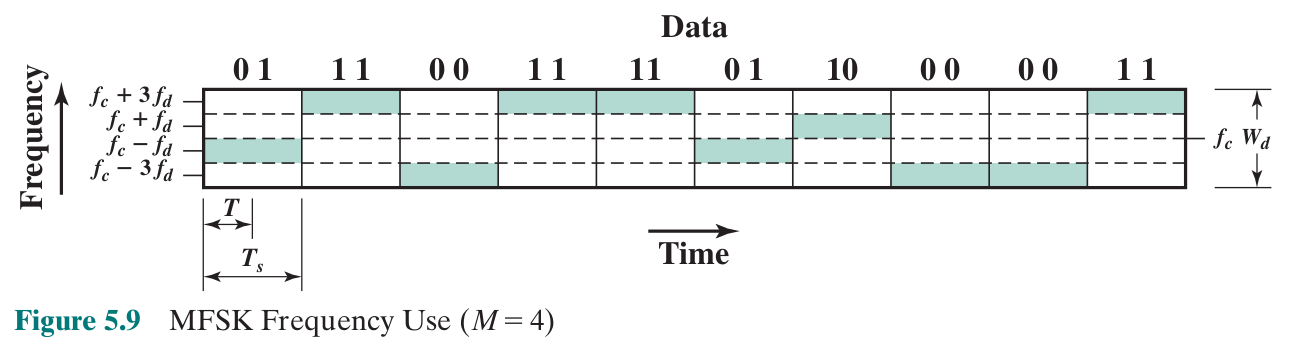
\includegraphics[width=\linewidth]{img/img13}
	\end{center}
\end{frame}

\begin{frame}
	\frametitle{Phase Shift Keying (PSK)}
	\begin{itemize}
		\item The phase of the carrier signal is shifted to represent data
		\item Binary PSK
		\begin{itemize}
			\item Two phases represent the two binary digits
		\end{itemize}
		\item Differential PSK
		\begin{itemize}
			\item Phase shifted relative to previous transmission rather than some reference signal
		\end{itemize}
	\end{itemize}
\end{frame}

\begin{frame}
	\begin{center}
		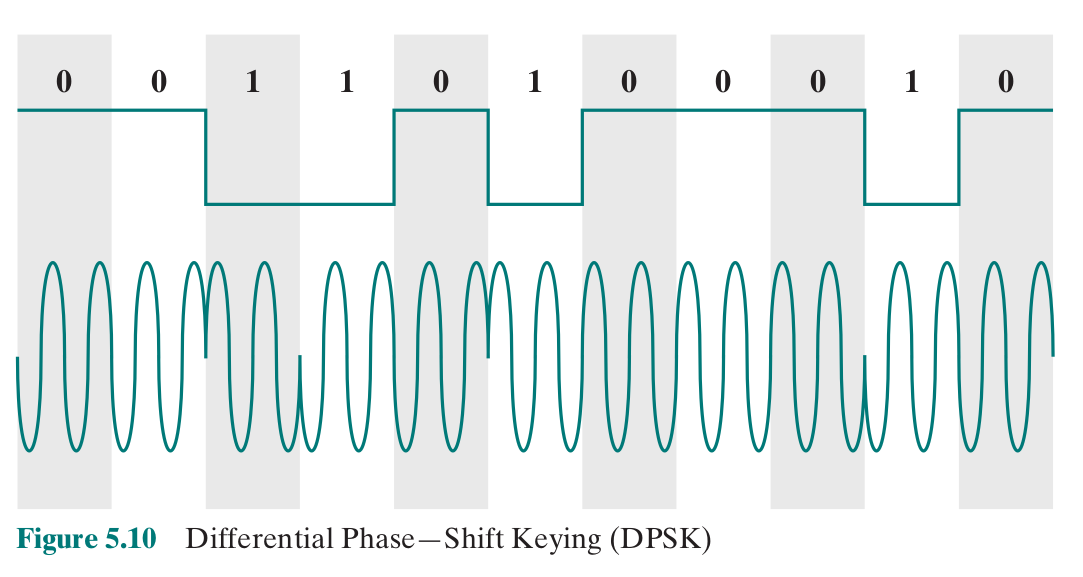
\includegraphics[width=\linewidth]{img/img14}
	\end{center}
\end{frame}

\begin{frame}
	\begin{center}
		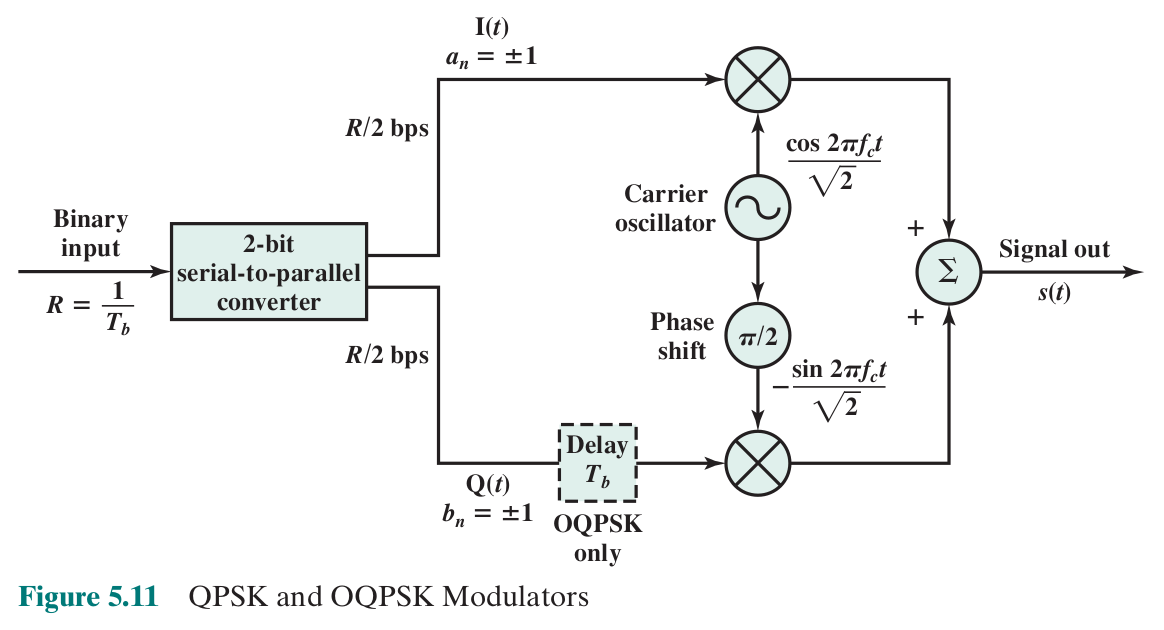
\includegraphics[width=\linewidth]{img/img15}
	\end{center}
\end{frame}

\begin{frame}
	\frametitle{Quadrature Phase Shift Keying\\(QPSK)}
	\begin{center}
		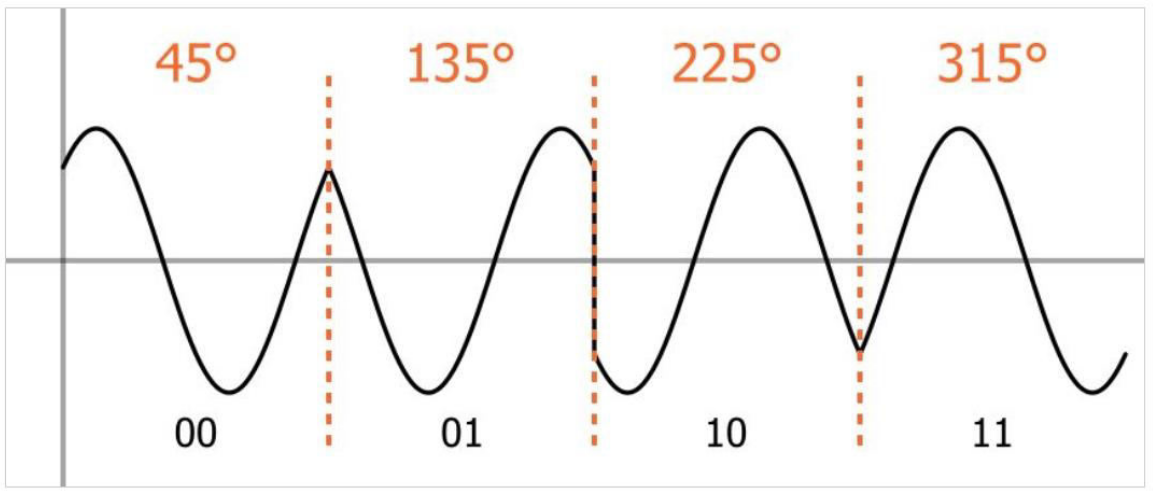
\includegraphics[width=\linewidth]{img/img16}
	\end{center}
\end{frame}

\begin{frame}
	\begin{center}
		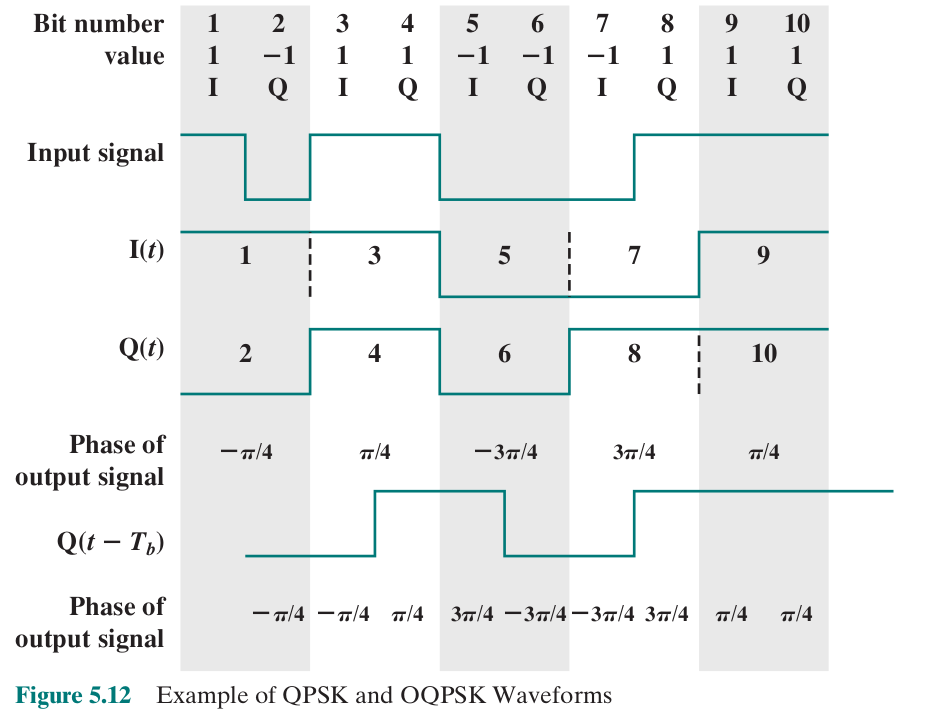
\includegraphics[width=0.8\linewidth]{img/img17}
	\end{center}
\end{frame}

\begin{frame}
	\begin{center}
		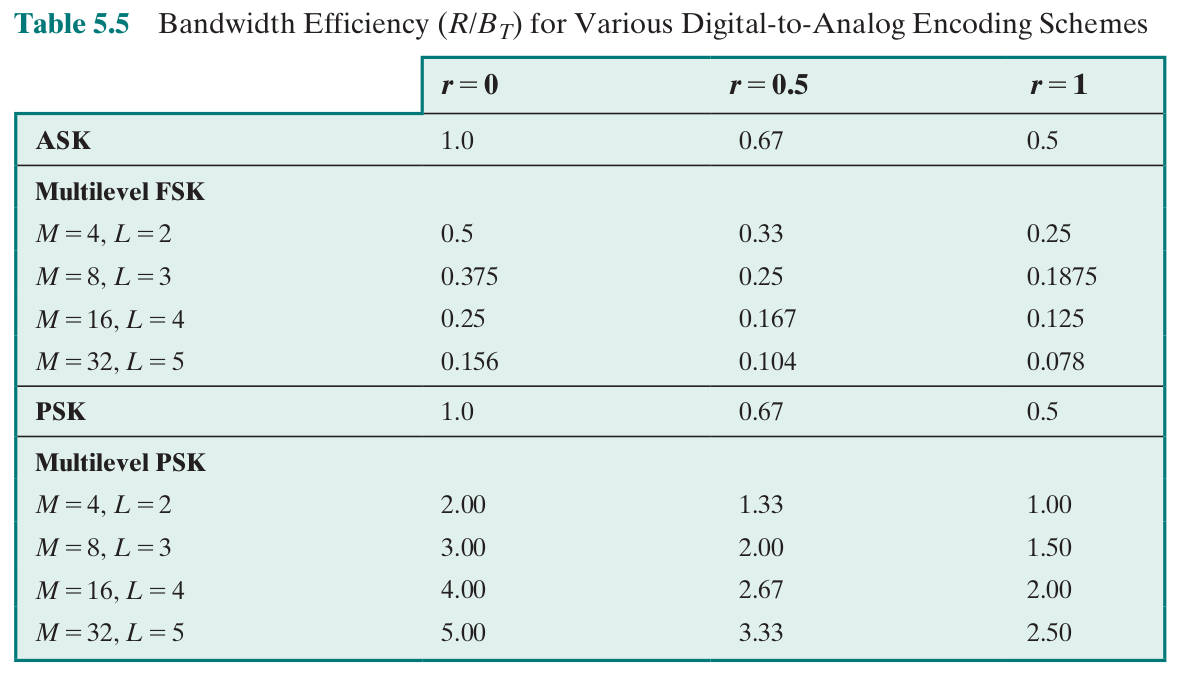
\includegraphics[width=\linewidth]{img/img18}
	\end{center}
\end{frame}

\begin{frame}
	\frametitle{Performance of Digital to Analog Modulation Schemes}
	\begin{multicols}{2}
		\centering \textbf{Bandwidth}
		\begin{itemize}
			\item ASK/PSK bandwidth directly relates to bit rate
			\item Multilevel PSK gives significant improvements
		\end{itemize}
		\vfill\null
		\columnbreak
		\centering \textbf{In presence of noise}
		\begin{itemize}
			\item Bit error rate of PSK and QPSK are about 3 dB superior to ASK and FSK
			\item MFSK and MPSK have tradeoff between bandwidth efficiency and error performance
		\end{itemize}
	\end{multicols}
\end{frame}

\begin{frame}
	\begin{center}
		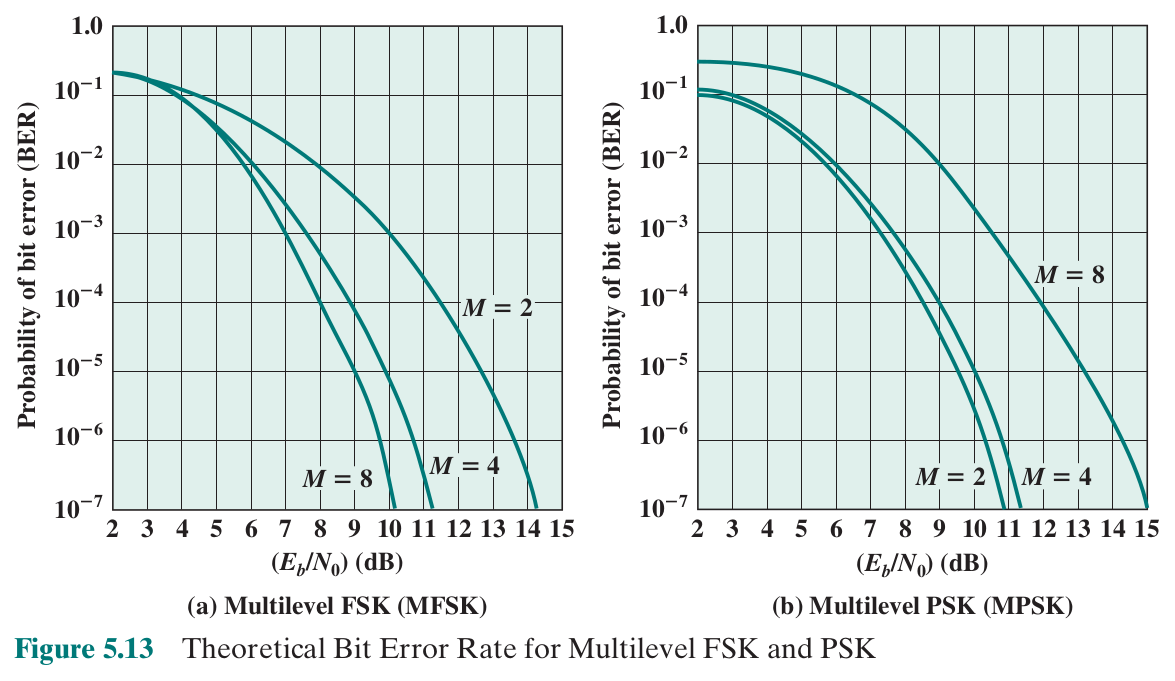
\includegraphics[width=\linewidth]{img/img19}
	\end{center}
\end{frame}

\begin{frame}
	\frametitle{Quadrature Amplitude Modulation (QAM)}
	\begin{itemize}
		\item QAM is used in the asymmetric digital subscriber line (ADSL), in cable modems, and in some wireless standards
		\item Is a combination of ASK and PSK
		\item Logical extension of QPSK
		\item Send two different signals simultaneously on the same carrier frequency
		\begin{itemize}
			\item Use two copies of carrier, one shifted 90$^{\circ}$
			\item Each carrier is ASK modulated
			\item Two independent signals simultaneously transmitted over the same medium
			\item At the receiver, the two signals are demodulated and the results are combined to produce the original binary input
		\end{itemize}
	\end{itemize}
\end{frame}

\begin{frame}
	\begin{center}
		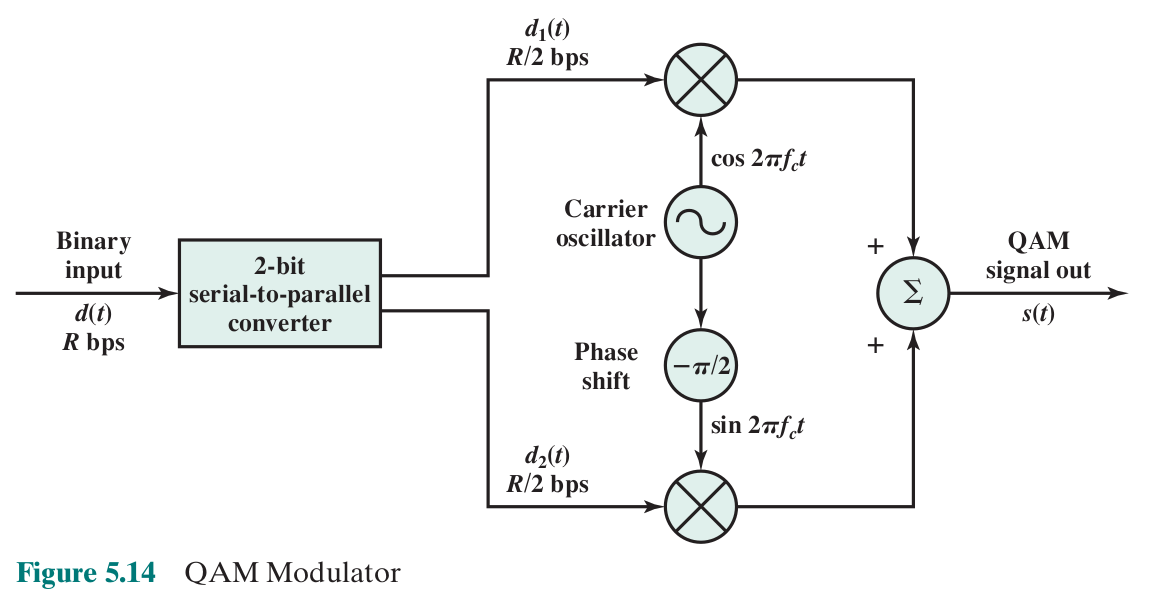
\includegraphics[width=\linewidth]{img/img20}
	\end{center}
\end{frame}

\begin{frame}
	\begin{center}
		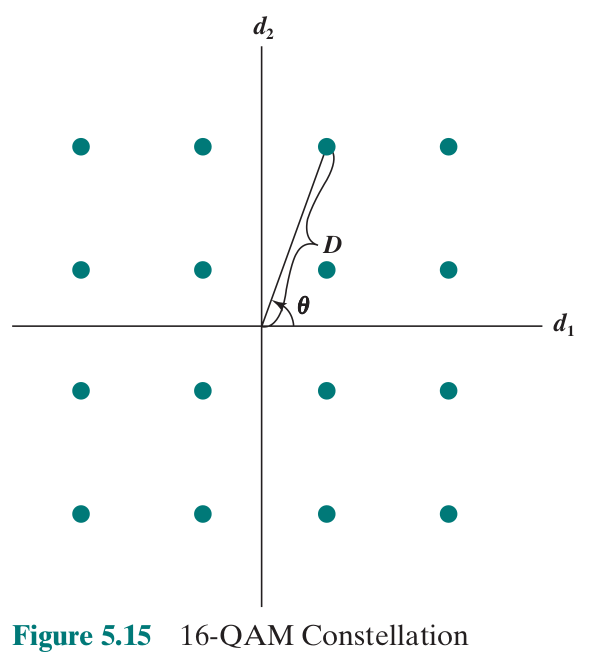
\includegraphics[width=0.5\linewidth]{img/img21}
	\end{center}
\end{frame}

\begin{frame}
	\begin{center}
		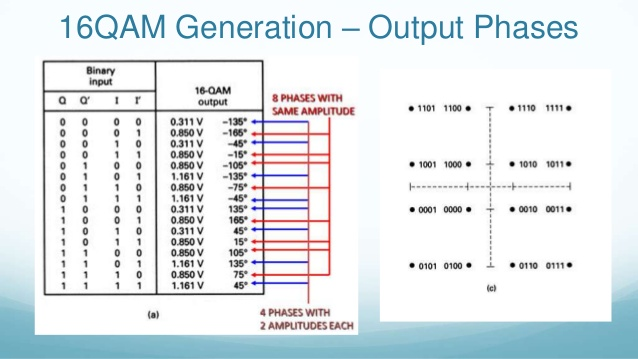
\includegraphics[width=\linewidth]{img/img22}
	\end{center}
\end{frame}

\begin{frame}
	\frametitle{Analog Data, Digital Signal}
	\begin{itemize}
		\item Digitization is the conversion of analog data into digital data which can then:
		\begin{itemize}
			\item Be transmitted using NRZ-L
			\item Be transmitted using code other than NRZ-L
			\item Be converted to analog signal
		\end{itemize}
		\item Analog to digital conversion is done using a codec
		\begin{itemize}
			\item Pulse code modulation
			\item Delta modulation
		\end{itemize}
	\end{itemize}
\end{frame}

\begin{frame}
	\begin{center}
		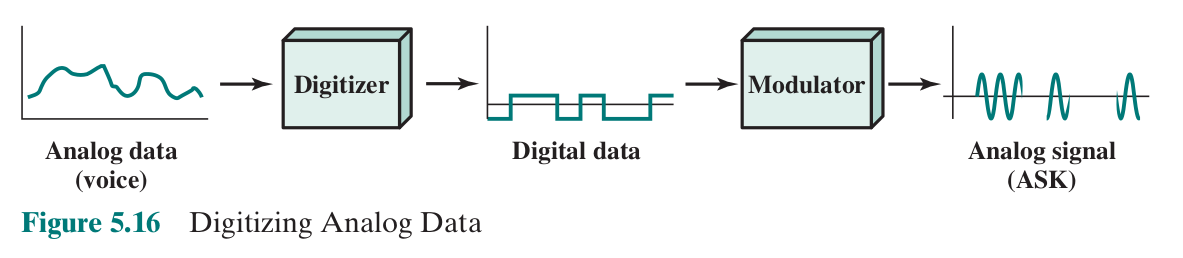
\includegraphics[width=\linewidth]{img/img23}
	\end{center}
\end{frame}

\begin{frame}
	\frametitle{Analog Data, Digital Signal}
	\begin{itemize}
		\item Based on the sampling theorem:
		\begin{itemize}
			\item “If a signal f(t) is sampled at regular intervals of time and at a rate higher than twice the highest signal frequency, then the samples contain all the information of the original signal. The function f(t) may be reconstructed from these samples by the use of a lowpass filter.”
		\end{itemize}
		\item Pulse Amplitude Modulation (PAM)
		\begin{itemize}
			\item Analog samples
			\item To convert to digital, each of these analog samples must be assigned a binary code
		\end{itemize}
	\end{itemize}
\end{frame}

\begin{frame}
	\begin{center}
		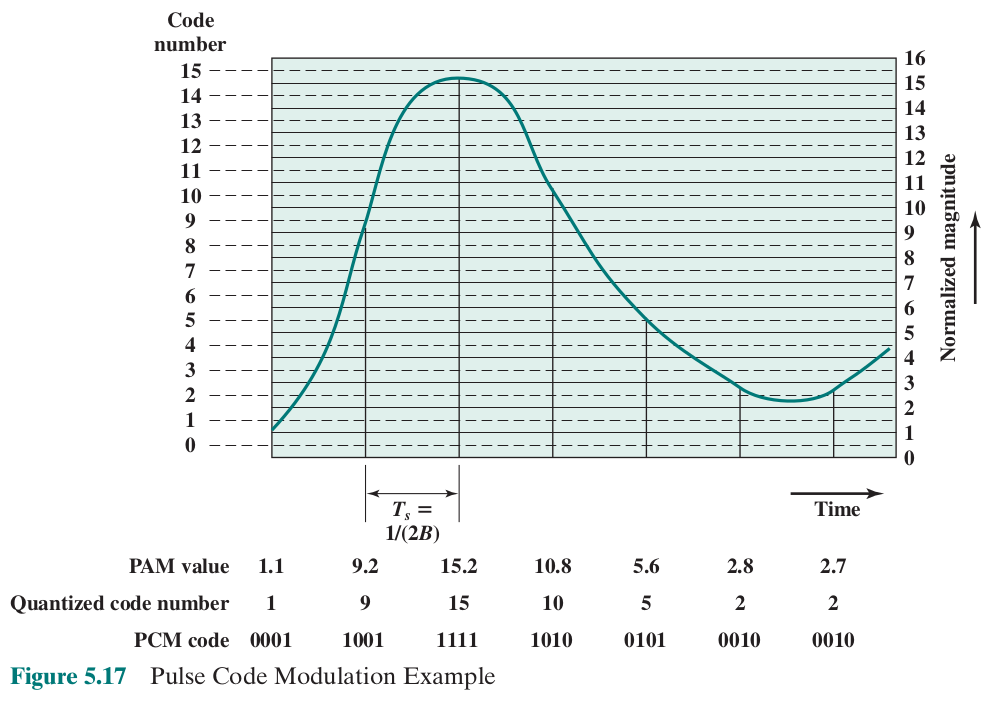
\includegraphics[width=0.9\linewidth]{img/img24}
	\end{center}
\end{frame}

\begin{frame}
	\begin{center}
		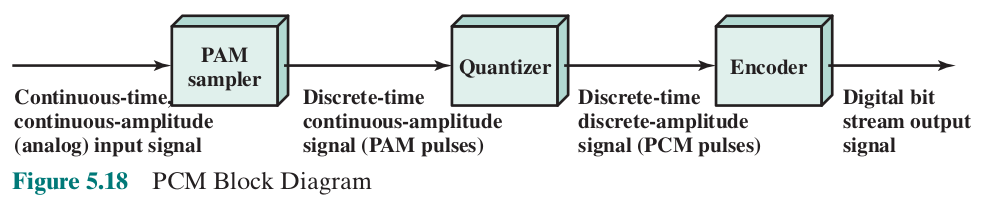
\includegraphics[width=\linewidth]{img/img25}
	\end{center}
\end{frame}

\begin{frame}
	\begin{center}
		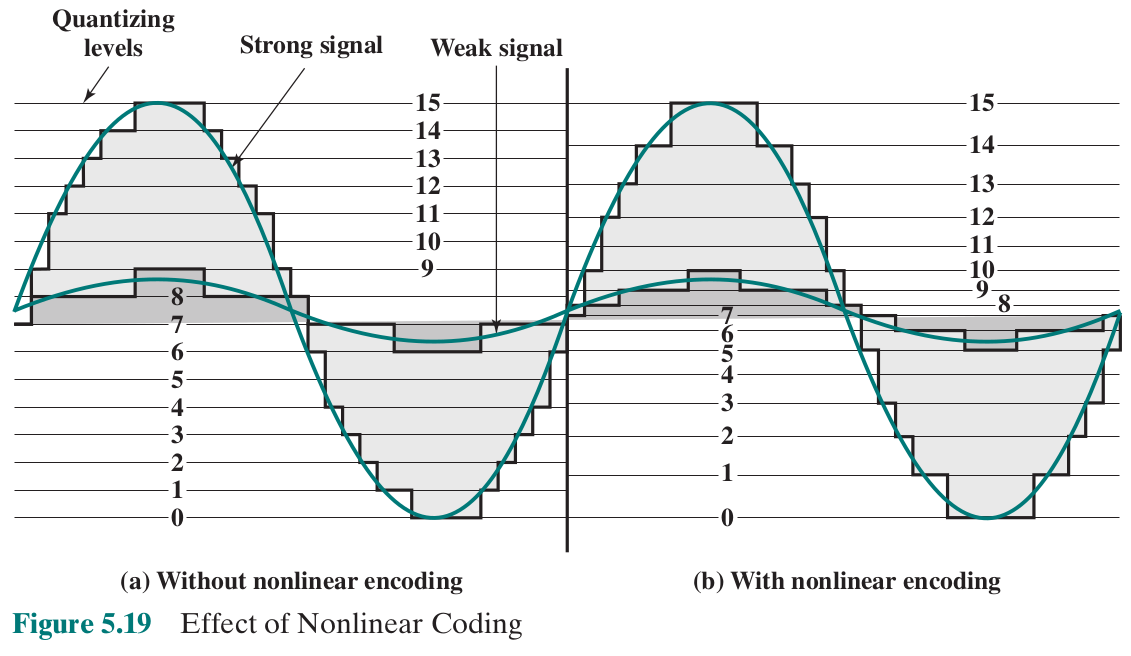
\includegraphics[width=\linewidth]{img/img26}
	\end{center}
\end{frame}

\begin{frame}
	\frametitle{Delta Modulation (DM)}
	\begin{itemize}
		\item Analog input is approximated by a staircase function
		\begin{itemize}
			\item Can move up or down one quantization level ($ \delta $) at each sampling interval
		\end{itemize}
		\item Has binary behavior
		\begin{itemize}
			\item Function only moves up or down at each sampling interval
			\item Output of the delta modulation process can be represented as a single binary digit for each sample
			\item 1 is generated if the staircase function is to go up during the next interval, otherwise a 0 is generated
		\end{itemize}
	\end{itemize}
\end{frame}

\begin{frame}
	\begin{center}
		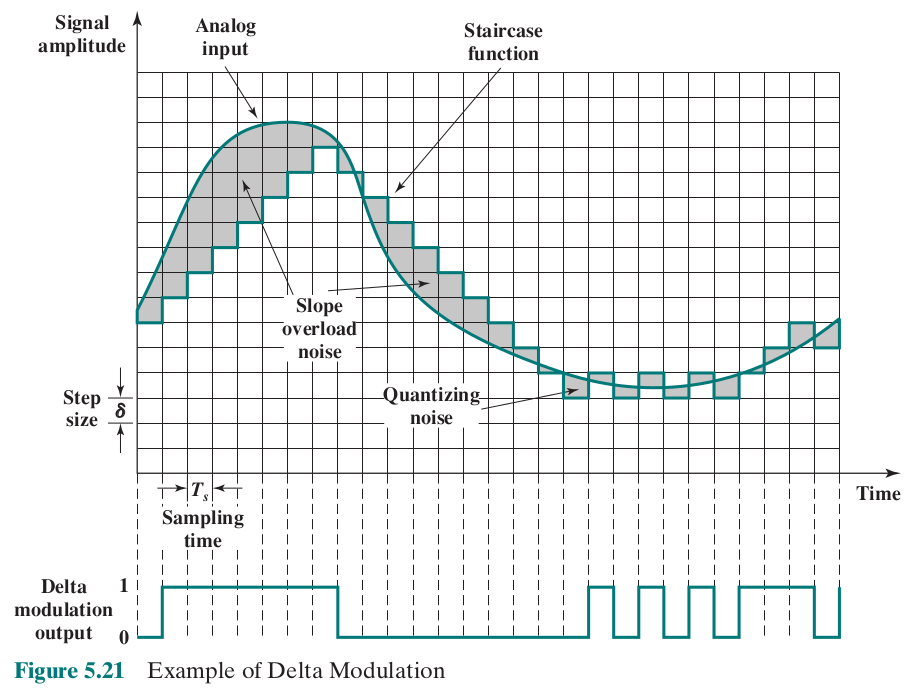
\includegraphics[width=0.9\linewidth]{img/img27}
	\end{center}
\end{frame}

\begin{frame}
	\begin{center}
		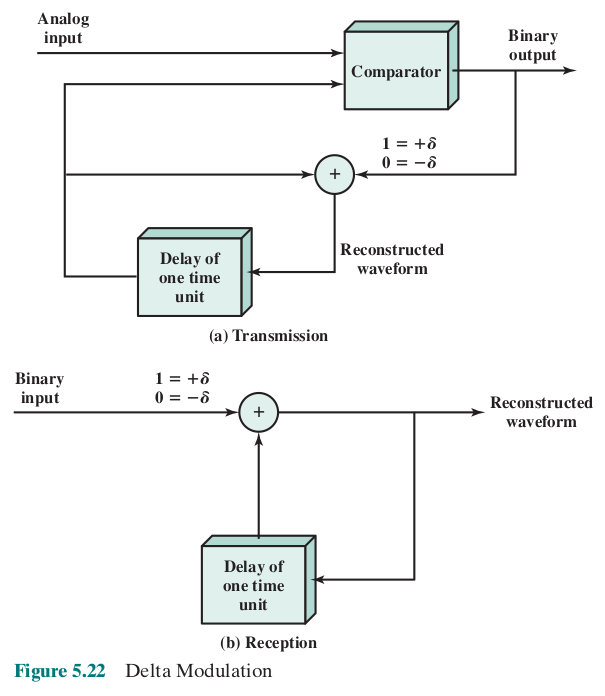
\includegraphics[width=0.6\linewidth]{img/img28}
	\end{center}
\end{frame}

\begin{frame}
	\frametitle{Summary}
	\begin{multicols}{2}
		\begin{itemize}
			\item Digital data, digital signals
			\begin{itemize}
				\item Nonreturn to zero (NRZ)
				\item Multilevel binary
				\item Biphase
				\item Modulation rate
				\item Scrambling techniques
			\end{itemize}
			\item Analog data, digital signals
			\begin{itemize}
				\item Pulse code modulation
				\item Delta modulation (DM)
				\item Performance
			\end{itemize}
			\columnbreak
			\item Digital data, analog signals
			\begin{itemize}
				\item Amplitude shift keying
				\item Frequency shift keying
				\item Phase shift keying
				\item Performance
				\item Quadrature amplitude modulation
			\end{itemize}
		\vfill\null
		\end{itemize}
	\end{multicols}
\end{frame}

%-----------------------
%  Tugas
%-----------------------

\begin{frame}
	\frametitle{Tugas Mandiri}
	\begin{itemize}
		\item Stallings, W. (2014). Data and Computer Communications, 10th Edition, New Jersey: Upper Saddle River\\
		\begin{itemize}
			\item Chapter 5 Signal Encoding Techniques
		\end{itemize}
		\item Gupta, P. C. (2006). Data Communications and Computer Networks. New Delhi: Prentice Hall of India\\
		\begin{itemize}
			\item Section 1.5 Digital Signal Encoding
			\item Section 1.6 Unipolar and Polar Line Codes
			\item Section 1.7 Bipolar Line Codes
			\item Section 4.1 Digital Modulation Methods
			\item Section 4.2 Multilevel Modulation
			\item Section 4.3 Differential PSK
		\end{itemize}
		\item Tanenbaum, A. S. \& Wetherall, D. J. (2013). Computer Networks, Fifth Edition. London: Pearson.\\
		\begin{itemize}
			\item Section 2.5 Digital Modulation and Multiplexing
		\end{itemize}
	\end{itemize}
\end{frame}

\begin{frame}
	\frametitle{Tugas Terstruktur}
	\textbf{Tampilkan Tugas 4}
\end{frame}

\end{document}
